\section{Results}
\subsection{Exact means and local calculations}
Table~\ref{tab:integrals} compares the four complete fitted-mean integrations with fresh simulations. The largest discrepancy is \MaxIntegralZ{} Monte Carlo standard errors. The first integral is $6.937226$, reproducing the value reported in the earlier draft through a newly implemented calculation. In the $\rho=.95$ configuration, the upper clipping mass is approximately $.384$; retaining it is consequential.

Whitening, determinant and directional-variance identities agree to floating-point precision on the checked matrix grid. Five deterministic $m=2$ population-curvature checks have maximum relative discrepancy \CurvatureError\%. These checks support the component expressions; they do not turn numerical agreement into a proof.

The finite-calibration integral also reveals a numerical limit. At the most extreme tested finite rank, $m=2,n=9,k=9$, a 512-point Jacobi rule still differs from adaptive integration by \MaxJacobiError\%. The expectation is finite, but its inverse-CDF integrand is singular at one. The default software utility therefore uses adaptive tail integration, and exposes Jacobi quadrature only as an explicit option with refinement guidance.

An additional fitting diagnostic evaluates $N\E(\widehat\rho-\rho)^2$ against $d\kappa/m$. At $N=500$ and $\kappa=1$ or 1.5, the estimates are near the limiting values. At $\kappa=3$, the discrepancies remain substantial: $.2174$ versus $.2700$ for $m=4$, and $.0756$ versus $.0900$ for $m=12$. The expansion is consequently unsuitable as an unchecked finite-sample equality under stronger scale heterogeneity. Figure~\ref{fig:costs} reports this diagnostic alongside calibration costs.

\begin{table*}[t]
\centering\small
\caption{Complete fitted-mean checks, all at $m=2$ and unit test scale. Each Monte Carlo estimate uses 30,000 independent fits. Refinement is the absolute change when all integration grids are increased. Training scales, respectively: $(.7,1.3)$, $(1,1)$, $(.5,1,1.5,2)$, $(.5,1,1.5,2)$.}
\label{tab:integrals}
\begin{tabular}{rrrrrrrr}
\toprule
$\rho$ & $N$ & $n$ & Integral & MC mean & MC SE & Refinement & Discrepancy / SE \\
\midrule
0.40 & 2 & 19 & 6.9372 & 6.9633 & 0.0261 & 0.0039 & 1.00 \\
0.80 & 2 & 49 & 3.8420 & 3.8527 & 0.0076 & 0.0007 & 1.41 \\
0.95 & 4 & 19 & 2.1708 & 2.1648 & 0.0073 & 0.0013 & -0.82 \\
-0.40 & 4 & 49 & 5.6455 & 5.6506 & 0.0112 & 0.0003 & 0.45 \\
\bottomrule
\end{tabular}

\end{table*}

\begin{figure*}[t]
\centering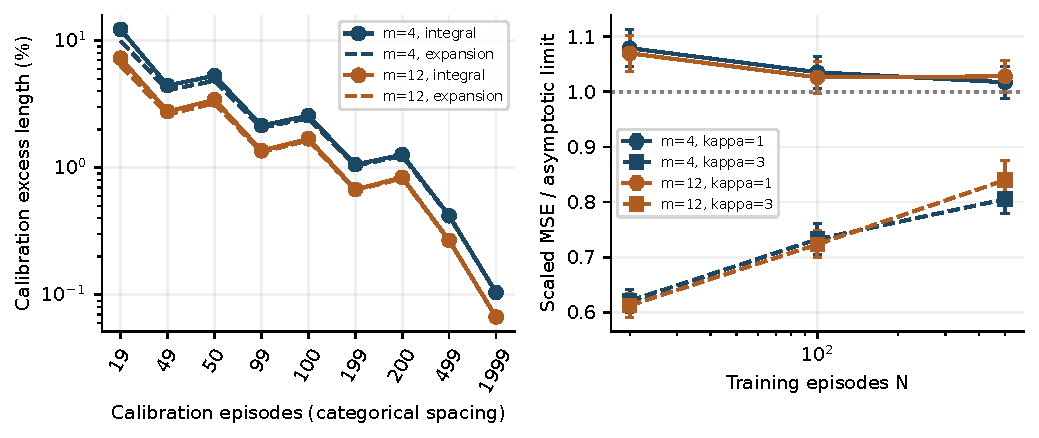
\includegraphics[width=.96\textwidth]{figures/finite_costs.pdf}
\caption{Left: known-coefficient finite-calibration excess length and its leading approximation, retaining integer-rank rounding. Adjacent calibration sizes have categorical spacing. Right: empirical scaled coefficient MSE divided by its asymptotic limit; 10,000 fitted samples per point, with 95\% Monte Carlo intervals. Stronger amplitude heterogeneity causes a material finite-sample discrepancy.}
\label{fig:costs}
\end{figure*}

\subsection{Common Gaussian dynamics}
Table~\ref{tab:common} reports actual coverage and widths for every specified comparator. IN-ARCP's mean-length ratios to the invariant Ad-EffOrt implementation are \AdaptFour{} and \AdaptTwelve{} at $m=4$ and 12. Its ratios to the same-fit Student reference are \StudentFour{} and \StudentTwelve{}, with paired Monte Carlo intervals containing one. The results therefore support efficiency relative to the particular invariant learned comparator while showing near parity with the classical reference.

Against native Ad-EffOrt, the corresponding ratios are \NativeFour{} and \NativeTwelve{}. The $m=4$ result favors the native procedure under unchanged amplitudes. The raw-RMS ablation is longer in both history settings, indicating a benefit from accounting for correlation in the history scale while holding the AR center fixed. Figure~\ref{fig:comparisons} retains all these comparisons.

\begin{table*}[t]
\centering\small
\caption{Fresh common-Gaussian AR(1) comparisons, unchanged amplitude distribution. $N=500,n=499,\alpha=.1$; 100 independent fits per history length. Widths are in the generator's response units. Full per-fit outcomes and Monte Carlo standard errors are supplied.}
\label{tab:common}
\begin{tabular}{lrrrr}
\toprule
Method & Coverage, $m=4$ & Length, $m=4$ & Coverage, $m=12$ & Length, $m=12$ \\
\midrule
IN-ARCP & 0.8985 & 2.318 & 0.8991 & 2.008 \\
AR + raw-RMS & 0.8998 & 2.799 & 0.8986 & 2.253 \\
AR + global & 0.8978 & 1.933 & 0.8972 & 1.923 \\
Student & 0.8988 & 2.309 & 0.9006 & 2.012 \\
Ad-EffOrt native & 0.8975 & 2.017 & 0.8975 & 2.044 \\
Ad-EffOrt invariant & 0.9002 & 2.774 & 0.9001 & 2.387 \\
CQR invariant & 0.8977 & 2.825 & 0.8985 & 2.358 \\
RF invariant & 0.8990 & 2.649 & 0.9001 & 2.318 \\
\bottomrule
\end{tabular}

\end{table*}
\begin{figure*}[t]
\centering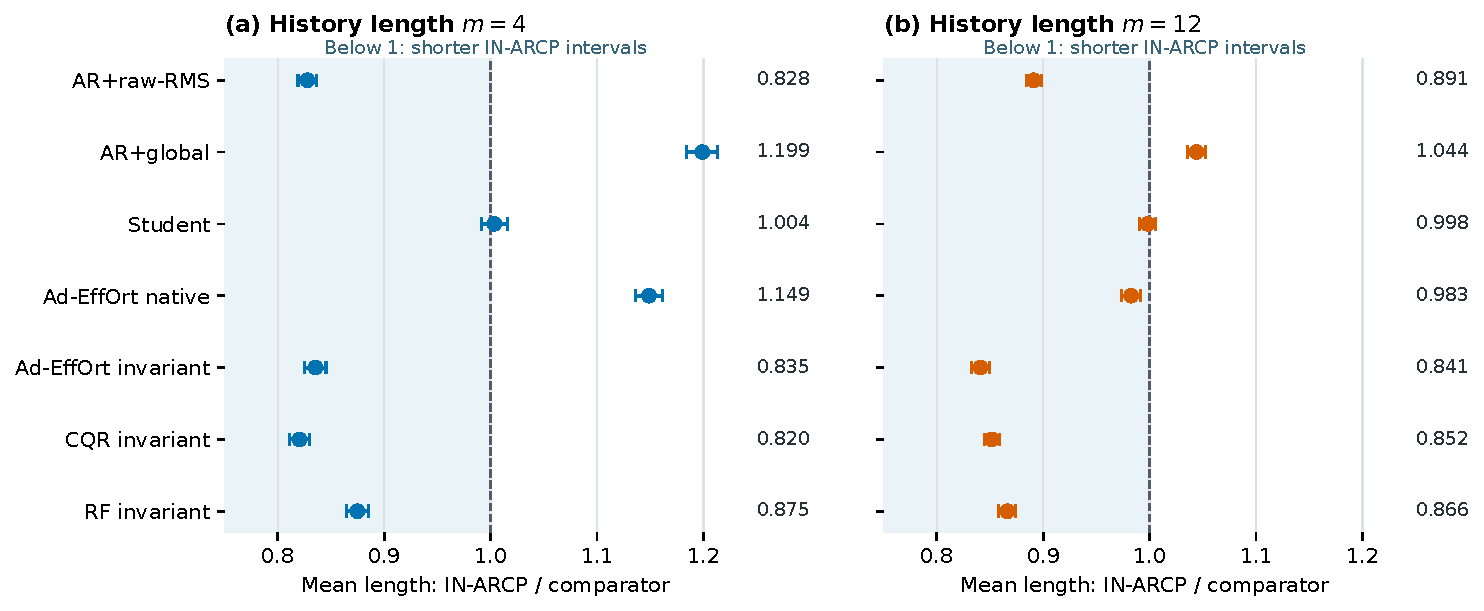
\includegraphics[width=.96\textwidth]{figures/comparisons.pdf}
\caption{Mean-length ratios in the common-Gaussian setting, with paired descriptive 95\% Monte Carlo intervals. Ratios below one favor IN-ARCP in mean length. All methods' coverage estimates are retained in Table~\ref{tab:common}; these comparisons concern fixed implementations and budgets.}
\label{fig:comparisons}
\end{figure*}

Additional implementation checks found numerical path sensitivity in the nonsmooth Ad-EffOrt optimizer. A post-validation Gaussian sensitivity study consequently compares both polynomial arithmetic forms and 1,000/2,000 updates, retaining every configuration. Across these settings, IN-ARCP's ratios to the invariant construction range from \OptInvMin{} to \OptInvMax{}; the native $m=4$ ratios range from \OptNativeMin{} to \OptNativeMax{}. The supplement reports all cells. This check qualifies the comparison as implementation-specific and does not establish exact optimizer equivalence or optimal tuning.

\subsection{Scale transfer and structural changes}
Whole-episode doubling leaves coverage of the invariant constructions unchanged and doubles their widths, as expected from homogeneity. Native Ad-EffOrt and global AR calibration lose coverage in that arm (Table~\ref{tab:shift}). Future-only doubling reduces IN-ARCP coverage to \FutureFour{} and \FutureTwelve{}. This is an expected boundary of the proposition, not a failure under its stated premise.

The structural challenges also produce meaningful losses. For independently varying episode coefficients, IN-ARCP has \VariableFour{} and \VariableTwelve{} times the mean length of the invariant nonlinear RF comparator at similar observed coverage. The direction of this result agrees with the limits of a shared linear center. In the heavy-tailed AR(1) setting, Student coverage is below the target, especially for $m=4$, while conformal calibration remains near the target. CQR, native/adapted Ad-EffOrt and all ablations remain in the complete result tables, including cases where they are shorter.

\begin{table*}[t]
\centering\small
\caption{Gaussian scale-transfer and negative-control coverage. The whole-episode arm rescales the same evaluation episodes. The future-only arm changes standardized shape and is outside the coverage premise.}
\label{tab:shift}
\begin{tabular}{llrrr}
\toprule
$m$ & Method & Unchanged & Whole episode $\times2$ & Future only $\times2$ \\
\midrule
4 & IN-ARCP & 0.8985 & 0.8985 & 0.5708 \\
4 & AR+global & 0.8978 & 0.6203 & 0.5377 \\
4 & Ad-EffOrt native & 0.8975 & 0.7016 & 0.5424 \\
12 & IN-ARCP & 0.8991 & 0.8991 & 0.5223 \\
12 & AR+global & 0.8972 & 0.6175 & 0.5350 \\
12 & Ad-EffOrt native & 0.8975 & 0.7470 & 0.5449 \\
\bottomrule
\end{tabular}

\end{table*}
\begin{table*}[t]
\centering\small
\caption{Structural challenges with unchanged marginal-scale distribution. Ratios are IN-ARCP mean length divided by invariant RF mean length. Whole-episode doubling gives identical coverage and ratios for both invariant methods. The Student column exposes sensitivity of the Gaussian threshold.}
\label{tab:structural}
\begin{tabular}{llrrrrr}
\toprule
Mechanism & $m$ & IN-ARCP cov. & RF cov. & Length ratio & 95\% MC interval & Student cov. \\
\midrule
AR(1), $t_5$ & 4 & 0.8991 & 0.8995 & 0.869 & [0.858, 0.880] & 0.8882 \\
AR(1), $t_5$ & 12 & 0.9029 & 0.9013 & 0.873 & [0.864, 0.881] & 0.8978 \\
AR(2) & 4 & 0.8983 & 0.8994 & 0.927 & [0.918, 0.935] & 0.9014 \\
AR(2) & 12 & 0.9004 & 0.9004 & 0.932 & [0.923, 0.941] & 0.8981 \\
Variable $\rho$ & 4 & 0.9008 & 0.8999 & 1.169 & [1.156, 1.182] & 0.9071 \\
Variable $\rho$ & 12 & 0.9020 & 0.9019 & 1.256 & [1.242, 1.270] & 0.8892 \\
\bottomrule
\end{tabular}

\end{table*}

\subsection{Allocation at a fixed budget}
The prespecified planning candidates reduce mean length relative to the equal $150/150$ split by \PlanOneGain\%{} for $\kappa=1$ and \PlanMixGain\%{} for $\kappa=1.5$ (Table~\ref{tab:planning}). The paired descriptive intervals lie below a ratio of one in these two evaluations.

The candidates lie near a broad group of efficient splits, rather than at a uniquely resolved empirical minimum. Some neighboring splits have slightly smaller sample means. Figure~\ref{fig:planning} displays every evaluated split and the discrepancy between the leading approximation and Monte Carlo means. These results validate a modest planning use of the theory under the tested parameters, not a general finite-sample optimum or a rule estimated from unknown real-world parameters.

\begin{table*}[t]
\centering\small
\caption{Prespecified allocation candidates versus equal allocation, total budget 300. Each ratio uses 1000 paired fitted repetitions. No empirical winner was selected after evaluating the test episodes.}
\label{tab:planning}
\begin{tabular}{rrrrr}
\toprule
$\kappa$ & Training & Calibration & Ratio to $150/150$ & 95\% MC interval \\
\midrule
1.0 & 61 & 239 & 0.9933 & [0.9889, 0.9978] \\
1.5 & 71 & 229 & 0.9944 & [0.9903, 0.9985] \\
\bottomrule
\end{tabular}

\end{table*}
\begin{figure*}[t]
\centering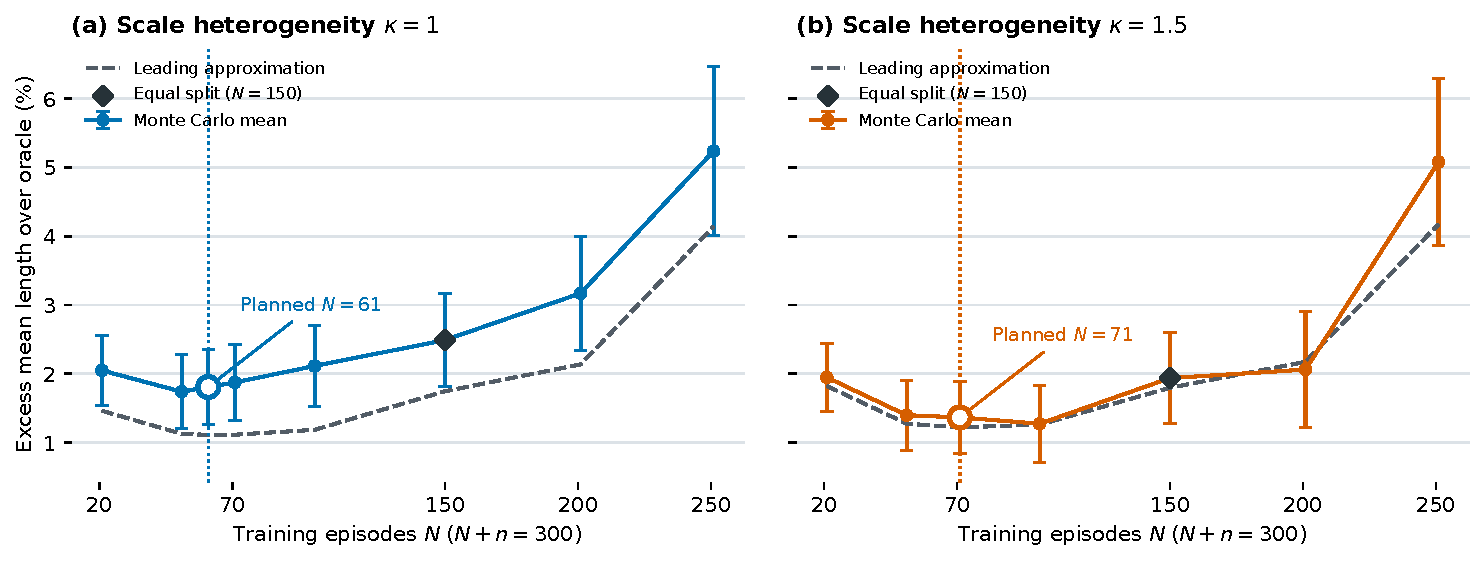
\includegraphics[width=.96\textwidth]{figures/planning.pdf}
\caption{Fixed-budget mean-length excess over the Gaussian equivariant oracle. Bars are descriptive 95\% Monte Carlo intervals for each mean, not paired differences. Dashed curves show the leading approximation; vertical dotted lines mark prespecified integer planning candidates.}
\label{fig:planning}
\end{figure*}
